\section[Introdução]{Introdução}

O projeto Vítimas de Crime teve como princípio garantir o direito à informação para vítimas de crime no estado do Rio Grande do Sul. A principal stakeholder do projeto era a promotora de justiça criminal de Viamão Dra. Márcia Vilanova.

Seu objetivo consistia no desenvolvimento de um aplicativo acessível às
vítimas, permitindo que estas alimentassem o sistema com provas e documentos de procedimentos criminais. Dessa forma, as informações seriam encaminhadas primeiro para a Polícia Civil e, posteriormente, para o Ministério Público, instruindo assim o processo. Especificamente, era vital garantir três pilares de direitos às vítimas: o Acesso à informação, a plena realização dos direitos e a devida proteção.

O primeiro pilar abrange esclarecimentos na plataforma virtual sobre o rito dos crimes comuns apenados com reclusão como roubo, furto, latrocínio ou estelionato, incluindo desde o registro de ocorrência policial até a conclusão do Inquérito Policial. Além disso, abrange leis especiais, como o estatuto do idoso e o estatuto da criança
e do adolescente.

O segundo pilar é dedicado ao exercício de direitos, envolvendo a prerrogativa de ser atendida, ouvida e a de buscar os órgãos de repressão do Estado. Este processo inclui fornecer informações detalhadas sobre contatos telefônicos e endereços, garantindo que as vítimas possam acessar de maneira efetiva e informada os recursos disponíveis as mesmas.

Por fim, o terceiro pilar visa buscar e garantir direitos de cidadania na rede municipal. Essa iniciativa aspira proporcionar atendimento médico, psiquiátrico e social para auxiliar na reestruturação da vida após o trauma causado pelo ilícito criminoso, incluindo considerações sobre mudanças de endereço, trabalho, escola, e outros aspectos relevantes para a reintegração plena da vítima na sociedade.

As datas de início e fim do projeto foram de 14/08/2023 a 20/11/2023 e contou com a orientação e suporte do prof. Dr. Daniel Callegari. A Figura 1 apresenta o time responsável pelo projeto.

\begin{figure}[H]
    \centering
    \small
    \caption{Time do projeto Vítimas de Crime}
    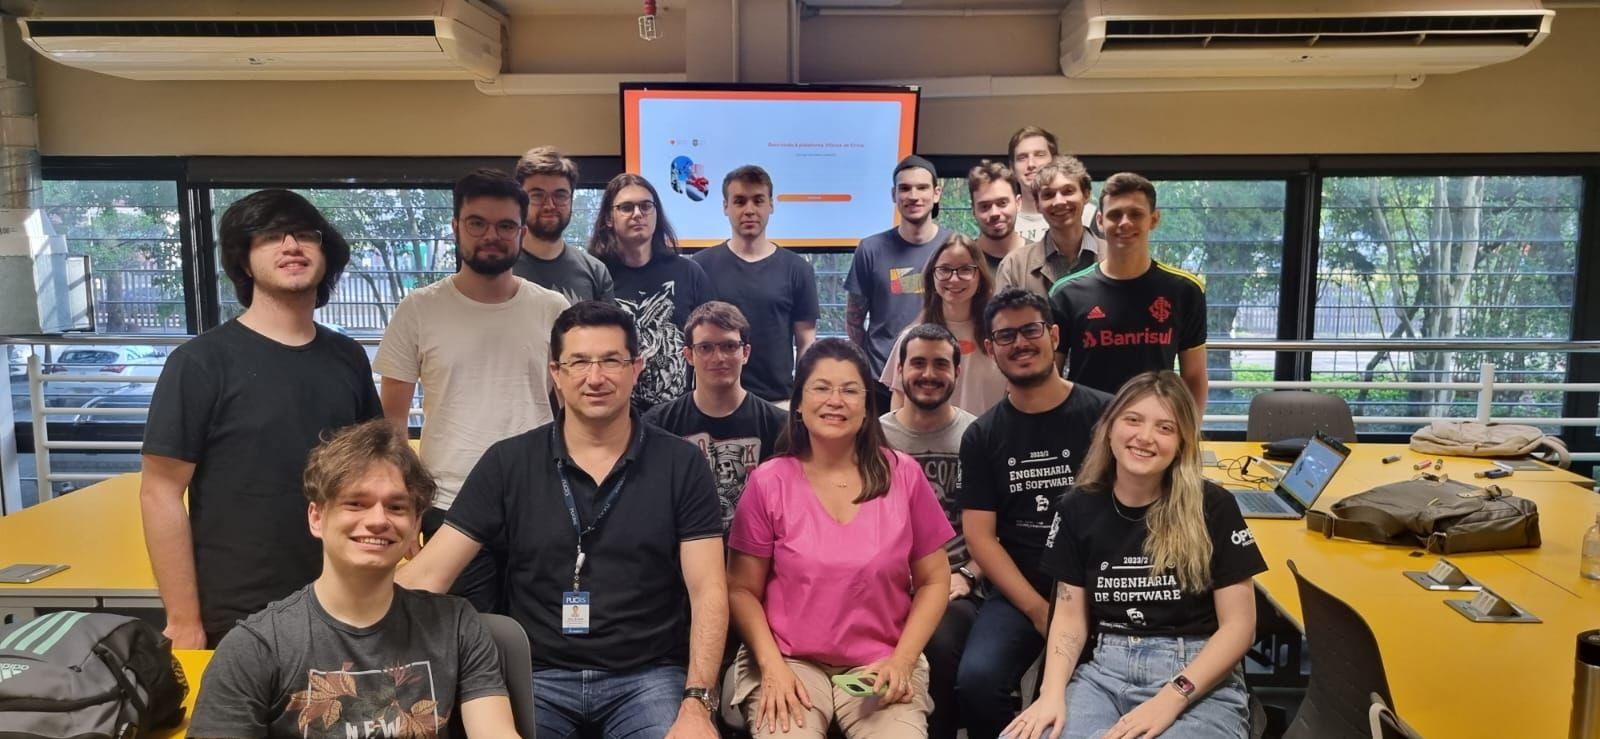
\includegraphics[width=1\linewidth]{conteudo//2 - ages I//conteudo//figures/figura1-time}
    Fonte: Autor
    \label{fig:projeto-time}
\end{figure}